\section{Digitaltechnik 1}
\subsection{Wahrheitstabelle, KDNF, KKNF, Y-Diagramm}
	\begin{tabular}{ll}
	  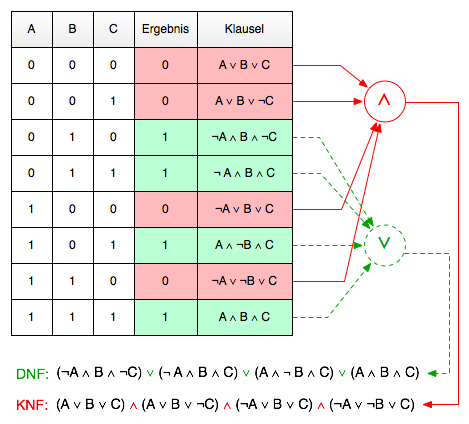
\includegraphics[width=0.4\textwidth]{pics/KNFDNF} &
	  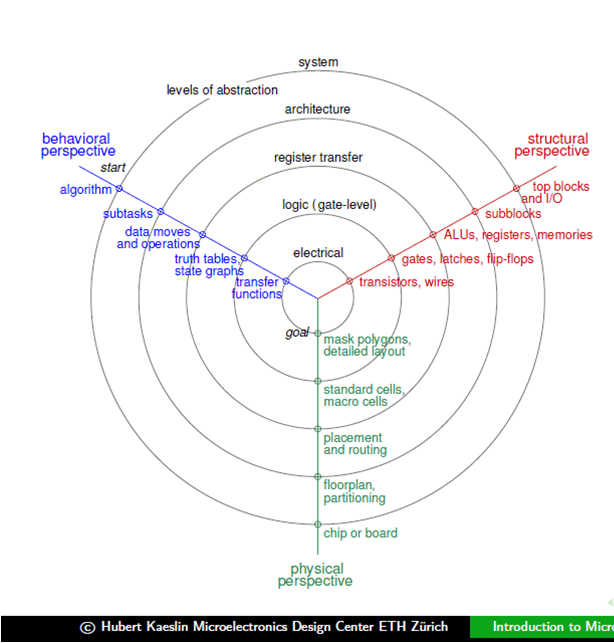
\includegraphics[width=0.3\textwidth]{pics/ydiagramm}
	\end{tabular}
	\\
	Kurzschreibweisen:\\
	KNF: $ a = \&([1],[2],3) $ \\
	DNF: $ b = \#([1],[3],37) $ \\
	Zeugs in eckigen Klammern bedeutet don't care.
\begin{multicols}{2}

\subsection{Karnaugh-Diagramm}
	\begin{tabular}{lll}
	  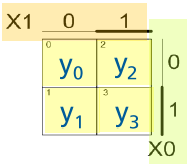
\includegraphics[width=0.1\textwidth]{pics/kv/2erKV} & 
	  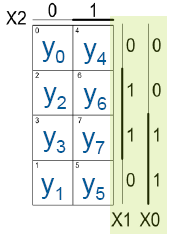
\includegraphics[width=0.1\textwidth]{pics/kv/3erKV} &
	  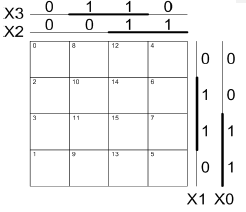
\includegraphics[width=0.2\textwidth]{pics/kv/4erKV}\\
	\end{tabular}
\subsection{Arbeiten mit KV-Diagramm}
	\begin{enumerate}
	\setlength{\itemsep}{1pt}
	  \setlength{\parskip}{0pt}
	  \setlength{\parsep}{0pt}
	\item Aufstellen der Wahrheitstabelle.\\
	\item "Ubertragen der Werte der Wahrheitstabelle in KV Diagramm.\\
	\item M"oglichst grosse Gruppen a $2^n$ Felder bilden.\\
	\item
	\begin{tabular}{p{4cm}p{4cm}}
	  DNF & KNF \\
	  Gruppen von Feldern mit Wert 1 oder d & Gruppen von Feldern mit Wert 0 oder d\\
	  Primimplikanten: AND Verkn�pfungen & Primimplikanten: OR Verkn�pfungen\\
	  OR Verkn�pfungen aller Primimpl. & AND Verkn�pfungen aller Primimpl.\\
	\end{tabular}
	\end{enumerate}

\end{multicols}
	\begin{tabular}{|c|c|c|c|c|c|c|c|c|}
	\hline
	Funktion & Buffer & NOT & AND & NAND & OR & NOR & EXOR & XNOR\\
	\hline
	Formel & a & $ \overline a $ & $ a \cdot b $ & $ \overline{a \cdot b} $ & $ a + b $ & $ \overline{a + b} $ & $ a \oplus b $ & $ \overline{a \oplus b} $\\
	& a & $ \overline a $ & $ a \wedge b $ & $ \overline{a \wedge b} $ & $ a \vee b $ & $ \overline{a \vee b} $ & $ a \not= b $ & $ \overline{a \not= b} $ \\
	& a & !a & $ a \& b $ & $ !(a \& b) $ & a\#b & !(a\#b) & a\$b & !(a\$b) \\
	%& & & & & & & $ a \veebar b $ & $ \overline{a \veebar b} $\\
	\hline
	& 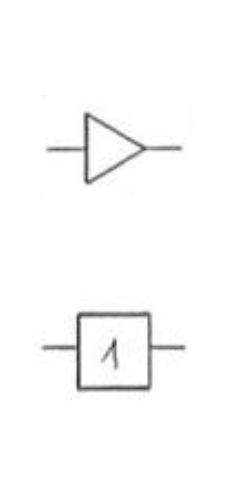
\includegraphics[width=0.04\textwidth]{pics/gates_symbol/buffer} &
	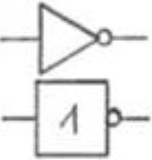
\includegraphics[width=0.04\textwidth]{pics/gates_symbol/not} & 
	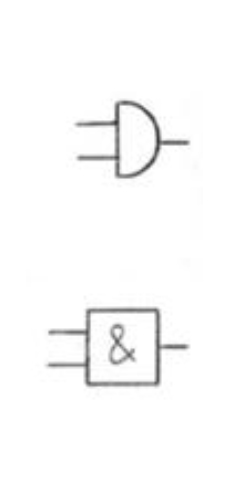
\includegraphics[width=0.04\textwidth]{pics/gates_symbol/and} & 
	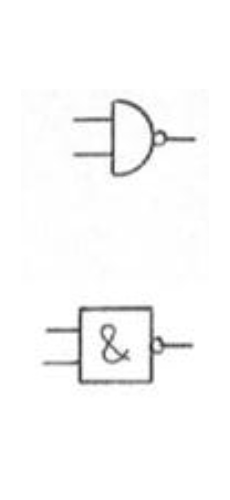
\includegraphics[width=0.04\textwidth]{pics/gates_symbol/nand} & 
	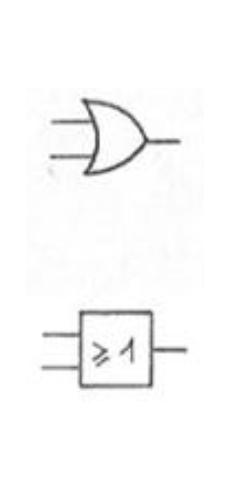
\includegraphics[width=0.04\textwidth]{pics/gates_symbol/or} & 
	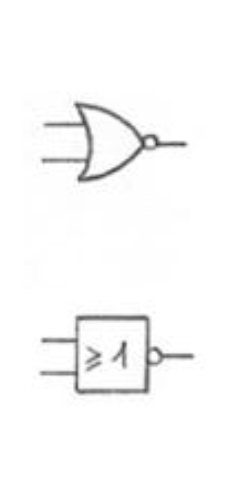
\includegraphics[width=0.04\textwidth]{pics/gates_symbol/nor} & 
	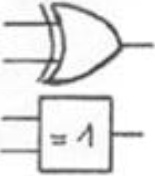
\includegraphics[width=0.04\textwidth]{pics/gates_symbol/exor} & 
	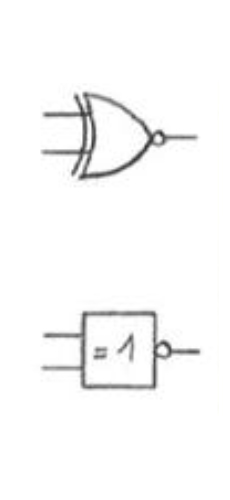
\includegraphics[width=0.04\textwidth]{pics/gates_symbol/xnor} \\
	\hline
	\#Trans & & 2 & 6 & 4 & 6 & 4 & 8 & \\
	\hline
\end{tabular}